\documentclass[border=10pt]{standalone}
\usepackage{tikz}
\usetikzlibrary{arrows.meta, positioning}
\usepackage{amsmath, amssymb}

\begin{document}
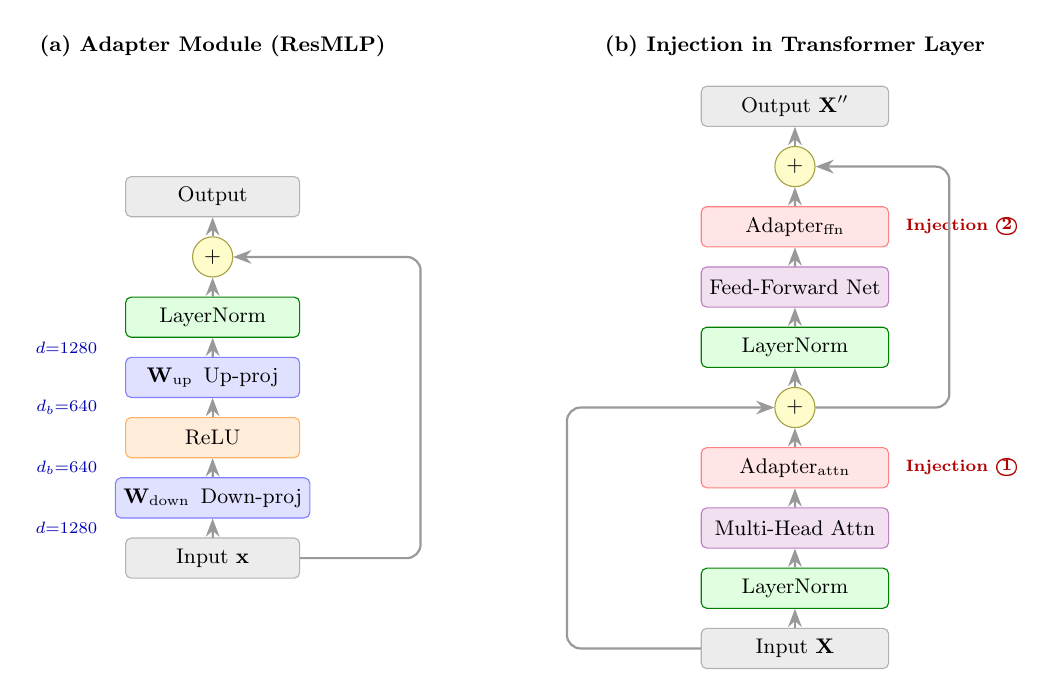
\begin{tikzpicture}[
    scale=0.85, every node/.style={transform shape},
    >=Stealth,
    box/.style={draw, rounded corners=2pt, minimum width=2.2cm, minimum height=0.6cm, align=center, font=\small},
    bluebox/.style={box, fill=blue!12, draw=blue!50},
    greenbox/.style={box, fill=green!12, draw=green!50!black},
    orangebox/.style={box, fill=orange!15, draw=orange!60},
    graybox/.style={box, fill=gray!15, draw=gray!60},
    redbox/.style={box, fill=red!10, draw=red!50},
    purplebox/.style={box, fill=violet!12, draw=violet!50},
    arr/.style={->, thick, draw=gray!80},
    dasharr/.style={->, thick, dashed, draw=gray!60},
    labelstyle/.style={font=\small\bfseries},
]

% ============ (a) Adapter Module Internal Structure ============
\begin{scope}[shift={(-4.2,1.35)}]
    \node[labelstyle] at (0, 7.65) {(a) Adapter Module (ResMLP)};

    \node[graybox, minimum width=2.6cm] (a_input) at (0, 0) {Input $\mathbf{x}$};

    \node[bluebox, minimum width=2.6cm] (a_wdown) at (0, 0.9) {$\mathbf{W}_{\mathrm{down}}$\, Down-proj};

    \node[orangebox, minimum width=2.6cm] (a_relu) at (0, 1.8) {ReLU};

    \node[bluebox, minimum width=2.6cm] (a_wup) at (0, 2.7) {$\mathbf{W}_{\mathrm{up}}$\, Up-proj};

    \node[greenbox, minimum width=2.6cm] (a_ln) at (0, 3.6) {LayerNorm};

    \node[draw, circle, minimum size=0.6cm, inner sep=0pt, fill=yellow!20, draw=yellow!60!black, font=\small\bfseries] (a_add) at (0, 4.5) {$+$};

    \node[graybox, minimum width=2.6cm] (a_output) at (0, 5.4) {Output};

    \draw[arr] (a_input) -- (a_wdown);
    \draw[arr] (a_wdown) -- (a_relu);
    \draw[arr] (a_relu) -- (a_wup);
    \draw[arr] (a_wup) -- (a_ln);
    \draw[arr] (a_ln) -- (a_add);
    \draw[arr] (a_add) -- (a_output);

    \draw[arr, rounded corners=5pt] (a_input.east) -- ++(1.8, 0) -- ++(0, 4.5) -- (a_add.east);

    \node[font=\scriptsize, text=blue!70!black, anchor=east] at (-1.6, 0.45) {$d{=}1280$};
    \node[font=\scriptsize, text=blue!70!black, anchor=east] at (-1.6, 1.35) {$d_b{=}640$};
    \node[font=\scriptsize, text=blue!70!black, anchor=east] at (-1.6, 2.25) {$d_b{=}640$};
    \node[font=\scriptsize, text=blue!70!black, anchor=east] at (-1.6, 3.15) {$d{=}1280$};
\end{scope}

% ============ (b) Transformer Layer Injection Position ============
\begin{scope}[shift={(4.5,0)}]
    \node[labelstyle] at (0, 9.0) {(b) Injection in Transformer Layer};

    \node[graybox, minimum width=2.8cm] (b_input) at (0, 0) {Input $\mathbf{X}$};

    \node[greenbox, minimum width=2.8cm] (b_ln1) at (0, 0.9) {LayerNorm};

    \node[purplebox, minimum width=2.8cm] (b_mha) at (0, 1.8) {Multi-Head Attn};

    \node[redbox, minimum width=2.8cm] (b_adp1) at (0, 2.7) {Adapter$_{\mathrm{attn}}$};

    \node[font=\scriptsize\bfseries, text=red!70!black] at (2.5, 2.7) {Injection \textcircled{\scriptsize 1}};

    \node[draw, circle, minimum size=0.6cm, inner sep=0pt, fill=yellow!20, draw=yellow!60!black, font=\small\bfseries] (b_add1) at (0, 3.6) {$+$};

    \node[greenbox, minimum width=2.8cm] (b_ln2) at (0, 4.5) {LayerNorm};

    \node[purplebox, minimum width=2.8cm] (b_ffn) at (0, 5.4) {Feed-Forward Net};

    \node[redbox, minimum width=2.8cm] (b_adp2) at (0, 6.3) {Adapter$_{\mathrm{ffn}}$};

    \node[font=\scriptsize\bfseries, text=red!70!black] at (2.5, 6.3) {Injection \textcircled{\scriptsize 2}};

    \node[draw, circle, minimum size=0.6cm, inner sep=0pt, fill=yellow!20, draw=yellow!60!black, font=\small\bfseries] (b_add2) at (0, 7.2) {$+$};

    \node[graybox, minimum width=2.8cm] (b_output) at (0, 8.1) {Output $\mathbf{X}''$};

    \draw[arr] (b_input) -- (b_ln1);
    \draw[arr] (b_ln1) -- (b_mha);
    \draw[arr] (b_mha) -- (b_adp1);
    \draw[arr] (b_adp1) -- (b_add1);
    \draw[arr] (b_add1) -- (b_ln2);
    \draw[arr] (b_ln2) -- (b_ffn);
    \draw[arr] (b_ffn) -- (b_adp2);
    \draw[arr] (b_adp2) -- (b_add2);
    \draw[arr] (b_add2) -- (b_output);

    \draw[arr, rounded corners=5pt] (b_input.west) -- ++(-2.0, 0) -- ++(0, 3.6) -- (b_add1.west);

    \draw[arr, rounded corners=5pt] (b_add1.east) -- ++(2.0, 0) -- ++(0, 3.6) -- (b_add2.east);

\end{scope}

\end{tikzpicture}
\end{document}
